\chapter[Ranking Computer Vision Service Issues using Emotion]
{Ranking Computer Vision Service Issues using Emotion\pubfootnote{Cummaudo:2021semotion}}
\label{ch:semotion2021}
\graphicspath{{mainmatter/publications/figures/semotion2021/}}

\glsresetall

\def\SEMNumTotalPostsFromSO{1,425}
\def\SEMNumTotalNonNoisePosts{1,239}
\def\SEMNumBeyerClassificationsMade{1,825}
\def\SEMNumClassificationsFromBeyerNonIRRAnalysis{1,375}
\def\SEMNumClassificationsFromBeyerIRRAnalysis{450}
\def\SEMNumNoisyPosts{186}
\def\SEMNumEmoTxtClassifications{1,412}
\def\SEMNumEmotionsDetected{792}
\def\SEMNumNoEmotionsDetected{620}
\def\SEMNumIRRPostsTiedMajority{four}
\def\SEMNumQuestionsOneEmo{1,096}
\def\SEMNumQuestionsTwoEmo{114}
\def\SEMNumQuestionsThreeEmo{28}
\def\SEMNumQuestionsFourEmo{one}

\def\SEMPctNoEmotionAPIUsage{41.46\%}	
\def\SEMPctNoEmotionDiscrepancy{43.39\%}	
\def\SEMPctNoEmotionErrors{48.36\%}
\def\SEMPctNoEmotionReview{40.77\%}
\def\SEMPctNoEmotionConceptual{43.66\%}	
\def\SEMPctNoEmotionAPIChange{31.25\%}
\def\SEMPctNoEmotionAverage{42.10\%}

\def\SEMPctFearAverage{16.77\%}
\def\SEMPctJoyAverage{8.85\%}
\def\SEMPctLoveAverage{8.15\%}
\def\SEMPctSadnessAverage{4.53\%}
\def\SEMPctSurpriseAverage{14.82\%}
\def\SEMPctAngerAverage{4.77\%}
\def\SEMPctNoEmotionAverage{42.10\%}

\begin{abstract}
Software developers are increasingly using cloud-based services that provide machine learning capabilities to implement `intelligent' features. Studies show that incorporating \glslong{ml} into an application increases technical debt, creates data dependencies, and introduces uncertainty due to their non-deterministic behaviour. We know very little about the emotional state of software developers who have to deal with such issues; and the impacts on productivity. This paper presents a preliminary effort to better understand the emotions of developers when experiencing issues with these services with the wider goal of discovering potential service improvements. We conducted a landscape analysis of emotions found in \SEMNumTotalPostsFromSO{} \glslong{so} questions about a specific and mature subset of these cloud-based services, namely those that provide computer vision techniques. To speed up the emotion identification process, we trialled an automatic approach using a pre-trained emotion classifier that was specifically trained on \glslong{so} content, EmoTxt, and manually verified its classification results. We found that the identified emotions vary for different types of questions, and a discrepancy exists between automatic and manual emotion analysis due to subjectivity.
\end{abstract}
\glsresetall
\glsunset{api}

\section{Introduction}
\label{semotion2021:sec:introduction}

Recent advances in \glslong{ai} have provided software engineers with new opportunities to incorporate complex \gls{ml} capabilities, such as computer vision, using cloud-based \glspl{iws}. 
However, the machine-learnt behaviour of these services is  non-deterministic and, given the dimensions of data used, their internal inference process is hard to reason about~\citep{Cummaudo:2019icsme}. Recent works show that developers struggle to use these services given that they are still in a nascent stage~\citep{Cummaudo:2020icse}, infusing machine learnt behaviour to a system often results in ongoing maintenance concerns~\citep{Sculley2015}. Further, the services' documentation fails to address common issues faced~\citep{Cummaudo:2020icse}.
Thus, developers resort to online communication---such as \gls{so}---to ask questions about their concerns, often expressing emotions such as frustration. Negative emotions have adverse effects to productivity \citep{wrobel2013}, and emotions expressed by developers online have been explored~\citep{ortu2016} including on \gls{so}~\citep{novielli2018, calefato2018}. 
There is a need to better understand emotions expressed by developers when using these services; such insight could be useful in assisting cloud vendors to make improvements that would generate the most value (e.g., overall service/\glsac{api} design, documentation of the services, clarification in error messages).

In our recent work~\citep{Cummaudo:2020icse}, we classified the \textit{types of issues} developers face when using these services, specifically \glspl{cvs}, by analysing \SEMNumTotalPostsFromSO{} \gls{so} questions using \citeauthor{Beyer:2018fm}'s taxonomy~\citep{Beyer:2018fm} (see \cref{semotion2021:tab:taxonomies}). This study extends our previous work by classifying the \textit{types of emotions} expressed in these questions, and to understand what types of questions express the strongest emotions. This serves as an initial step to formulate a prioritised set of improvements \gls{cvs} vendors can adopt that would bring the most value to developers (based on the types of issues developers express the strongest emotions about, thereby affecting their productivity). Motivated by existing studies exploring how emotions affect productivity~\citep{murgia2014, ortu2016, gachechiladze2017}, we identify the emotion(s) in each \gls{so} question (if any), and investigate whether the distribution of these emotions are similar across the various types of questions.

To achieve this goal, we opted for both \textit{automatic} and \textit{manual} classification approaches. Firstly, we used a pre-trained machine learnt emotion classifier, EmoTxt~\citep{novielli2018, calefato2018, calefato2017}, trained specifically on \gls{so} posts and grounded on an emotion classification model \citep{shaver1987}. To our knowledge, EmoTxt is the only emotion classifier trained on \gls{so} data and is well-documented for this purpose. We then triangulated the emotions detected by EmoTxt for each post against the question types we classified in \citep{Cummaudo:2020icse}. Given the subjective nature of emotions, we also \textit{manually} classified a representative sample of 300 posts using the same guidelines used to annotate the EmoTxt training dataset \citep{novielli2018}, thereby assessing overall agreement between different human raters, and manual (human) classification versus automatic (EmoTxt) classification. The three key contributions of our study are: 
\begin{enumerate}[label=(\roman*)]
    \item we find the distribution of emotions differs for the type of question being asked; 
    \item our analysis of the EmoTxt results when compared with manual efforts suggests that the classification model does not generalise the \gls{cvs} domain well; 
    \item we provide a complete replication package for future research, available at \url{https://bit.ly/2RIGQ2N}.
\end{enumerate}


\section{Background}\label{semotion2021:sec:emotion-mining}

%Developing software raises various emotions in developers at different times, including enjoyment, frustration, satisfaction, even fear and rage \cite{wrobel2013,ortu2016,wrobel2020,calefato2017}.

Studies on the role of emotions within the workplace, including the software engineering domain, have established a correlation between emotion and productivity ~\citep{wrobel2013, wrobel2020}. Negative emotions impact productivity negatively, whilst positive emotions impact positively. Even though in Wrobel's study \citep{wrobel2013}, \textit{anger}, a negative emotion, was found to generate a motivating state to ``try harder'' in a subset of developers,  overall, \textit{anger} was still found to have a negative impact on productivity. In recent years, researchers have focused on identifying the emotions expressed by software engineers within communication channels such as JIRA to communicate with their peers ~\citep{murgia2014, ortu2016, gachechiladze2017, novielli2018}. Most of these studies make use of one of the well established emotion classification frameworks during their emotion mining process. For example, ~\citet{murgia2014} and~\citet{ortu2016} investigated the emotions expressed by developers within an issue tracking system, such as JIRA, by labelling issue comments and sentences written by developers using Parrott's emotion framework. %\citet{gachechiladze2017} applied the Shaver's emotion framework to detect anger expressed in comments written by developers in JIRA. 

In an attempt to automate the emotion mining process, the Collab team~\citep{calefato2017, novielli2018} extended the work done by~\citet{ortu2016} by developing an emotion mining toolkit, EmoTxt~\citep{calefato2017} based on a gold standard dataset collected from 4,800 \gls{so} posts (of type questions, question comments, answers, and answer comments). 12 graduate computer science students were recruited as raters to manually annotate these 4,800 \gls{so} posts using the Shaver's emotion model (love, joy, anger, sadness, fear and surprise~\citep{shaver1987}). The work conducted by the Collab team is most relevant to our study since their focus is on identifying emotion from \gls{so} posts and their classifier is trained on a large dataset of \gls{so} posts.

\section{Methodology}\label{semotion2021:sec:methodology}

As discussed in \cref{semotion2021:sec:introduction}, the wider aims of this work are to develop a prioritised set of possible improvements to \gls{cvs} design based on the types of issues developers express (on \gls{so}) with the strongest emotions. This study makes an initial step in that direction by first identifying \textit{what} emotions exist (if any). We formulate four RQs:

\def\SEMRQOne{What emotions, if any, exist in the language used in \gls{so} questions about \glspl{cvs}?}
\def\SEMRQTwo{Does the classification of emotions vary for different types of \gls{so} questions?}
\def\SEMRQThree{What level of agreement exists between manual and \textit{automatic classification} of emotions (using EmoTxt)?}
\def\SEMRQFour{What level of agreement exists between individual raters who \textit{manually classify} emotions?}
\begin{enumerate}[label=\textbf{[RQ\arabic*]}, leftmargin=2\parindent]
    \item \SEMRQOne{}
    \item \SEMRQTwo{}
    \item \SEMRQThree{}
    \item \SEMRQFour{}
\end{enumerate}

\subsection{Dataset}

This paper extends our existing work by utilising our previously curated dataset of \SEMNumTotalPostsFromSO{} \gls{so} questions on four popular \gls{cvs} providers.\footnote{\label{semotion2021:ftne:list-of-services}Google Cloud Vision, AWS Rekognition, Azure Vision, IBM Watson.} We select \glspl{cvs} as a \textit{concrete example} of \glspl{iws} due to their mature presence of these types of services available to developers (see \citep{Cummaudo:2020icse} and \cref{semotion2021:sec:threats}). Each question is classified a question type per the taxonomy prescribed in \citet{Beyer:2018fm} (for reference, we provide our interpretation of this taxonomy within \cref{semotion2021:tab:taxonomies}). For further details on how this dataset was produced, we refer to the original paper~\citep{Cummaudo:2020icse}.

After performing additional cleansing of this dataset (to remove noise), we performed \textit{both} automatic and manual emotion classification based on \citeauthor{shaver1987}'s emotion taxonomy \citep{shaver1987}. Automatic emotion detection was performed using the EmoTxt classifier, and manual classification was performed by three co-authors on a sample of 300 posts. As this was a preliminary investigation, we iteratively explored several smaller representative samples to see if any emotions could be detected and agreed upon (see \cref{semotion2021:ssec:manual}). We calculated the inter-rater reliability between EmoTxt and our manually classified questions in two ways: (i)~to see the overall agreement between the three raters in applying the \citeauthor{shaver1987} emotions taxonomy, and (ii)~to see the overall agreement with EmoTxt's classifications. Additional dataset cleansing and results from manual and automatic emotion classification are available online at \url{https://bit.ly/2RIGQ2N}.

\begin{table*}[tb]
    \centering
    \caption[Our interpretations from a Stack Overflow question type taxonomy]{Descriptions of dimensions from our interpretation of \citeauthor{Beyer:2018fm}'s \gls{so} question type taxonomy.}
    \label{semotion2021:tab:taxonomies}
    \small
    \begin{tabular}{p{.2\linewidth}p{.75\linewidth}}
      \toprule
  
      \textbf{Dimension} & \textbf{Our Interpretation}
      \\
      \midrule
      
      \textbf{\glsac{api} usage\dotfill} &
      Issue on how to implement something using a specific component provided by the \glsac{api}
      \\
  
      \textbf{Discrepancy\dotfill} &
      The questioner's \textit{expected behaviour} of the \glsac{api} does not reflect the \glsac{api}'s \textit{actual behaviour}
      \\
  
      \textbf{Errors\dotfill} &
      Issue regarding an error when using the \glsac{api}, and provides an exception and/or stack trace to help understand why it is occurring
      \\
  
      \textbf{Review\dotfill} &
      The questioner is seeking insight from the developer community on what the best practices are using a specific \glsac{api} or decisions they should make given their specific situation
      \\
  
      \textbf{Conceptual\dotfill} &
      The questioner is trying to ascertain limitations of the \glsac{api} and its behaviour and rectify issues in their conceptual understanding on the background of the \glsac{api}'s functionality
      \\
  
      \textbf{\glsac{api} change\dotfill} &
      Issue regarding changes in the \glsac{api} from a previous version
      \\
  
      \textbf{Learning\dotfill} &
      The questioner is seeking for learning resources to self-learn further functionality in the \glsac{api}, and unlike discrepancy, there is no specific problem they are seeking a solution for
      \\
      \bottomrule 
    \end{tabular}
  \end{table*}

\subsection{Dataset Cleansing and Classifying Issue Types}
\label{semotion2021:ssec:method:filtering:classification}

As described in \citep{Cummaudo:2020icse}, the \SEMNumTotalPostsFromSO{} questions extracted were split into 5 random samples. The first author classified the first sample of  475 questions, with three other research assistants\footnote{Software engineers with at least two years industry experience.} classifying the remaining 900 questions over samples of 300 posts. The remaining 50 posts were used for reliability analysis, whereby these 50 posts were classified nine times by various researchers in our group, resulting in a total of \SEMNumClassificationsFromBeyerIRRAnalysis{} classifications for the 50 posts.

Each question was classified a question issue type (as described by \cref{semotion2021:tab:taxonomies}) or, where the question was a false-positive resulting from our original search query, we flagged the post as `noise' and removed them from further classification. \SEMNumNoisyPosts{} posts were flagged as noise, with a total of \SEMNumTotalNonNoisePosts{} were successfully classified a question type. To remove duplicates resulting from the reliability analysis, we applied a `majority rules' technique to each of these 50 posts, in which the issue type most consistent amongst the nine raters per question would win. (Given the nature of reliability analysis and assessment of subjectivity, each individual rater performed classifications in isolation, and as a result did not perform a reconciliation discussion as this would lead to changes to individual responses after-the-fact.) As an example, three raters classified a post as \textit{\glsac{api} Usage}, one rater classified the same post as a \textit{Review} question and \textbf{five} raters classified the post as \textit{Conceptual}. Therefore, the question was classified as a \textit{Conceptual} question. However, in \SEMNumIRRPostsTiedMajority{} cases, there was a tie in the majority. To resolve this, we used the issue type that was most classified within the 50 posts. For example, in another question, three raters each classified the same post as \textit{Discrepancy} and \textit{Errors}, while the remaining three raters flagged the post as noise. In this case, the tie was resolved down to \textit{Errors} as this classification received 72 more votes than \textit{Discrepancy} and 88 more votes than noisy posts across all classifications made in the sample of 50 posts. 

\subsection{Automatic Emotion Classification}

After all questions had been classified an issue type, we applied the method by~\citet{novielli2018} on our dataset consisting of questions only.
We started with a file containing the \SEMNumTotalNonNoisePosts{} non-noise \gls{so} questions, each with its associated question type given in \cref{semotion2021:tab:taxonomies}. We pre-processed this file by extracting the question ID and body text to meet the format requirements of the EmoTxt classifier~\citep{calefato2017}. This classifier was used as it was trained on \gls{so} posts as discussed in Section \cref{semotion2021:sec:emotion-mining}. We ran the classifier for each emotion as this was required by EmoTxt model. This resulted in six output prediction files (one file for each emotion: \textit{Love}, \textit{Joy}, \textit{Surprise}, \textit{Sadness}, \textit{Fear}, \textit{Anger}), which referenced a question ID and a binary value indicating emotion presence. We then merged these emotion prediction files into an aggregate file with question text and~\citeauthor{Beyer:2018fm}'s question type classifications that was performed in \citep{Cummaudo:2020icse}.

\subsection{Manual Emotion Classification} 
\label{semotion2021:ssec:manual}
\def\cohen{$C_{\kappa}$}
\def\light{$L_{\kappa}$}

In order to evaluate and also better understand the process used by EmoTxt to classify emotions, we randomly sampled 300 \gls{so} posts of various emotion annotations resulting from EmoTxt. Each of these 300 posts were classified by three raters (co-authors of this paper) who individually reviewed the question text against each of the six basic emotions~\citep{shaver1987} and flagged an emotion if deemed present, otherwise flagging \textit{No Emotion} instead. Each rater reviewed each question against the guidelines provided in \citep{novielli2018}. We then conducted reliability analysis of all three rater's results to measure the similarity in which independent raters classified each emotions against each \gls{so} post. Based on suggestions in \cite{Hallgren:2012kt}, we calculated Cohen's Kappa (\cohen{})~\citep{Cohen:1960tf} to measure the average inter-rater agreement \textit{between} pairs of raters, and then Light's Kappa (\light{})~\citep{Light:1971vz} to measure the \textit{overall} agreement amongst the three raters. Results are reported in \cref{semotion2021:tab:irr-results}. Initially, we had started with a manual classification of only 25 questions, however, this revealed strong disagreement among the three human raters. We extended the process to 150 questions and identified similar level of disagreements. We classified an additional 125 questions to conclude that the disagreements were persistent, and thus concluded manual classification at 300 posts.

\subsection{Comparing Manual and Automatic Classification Methods}

The next step involved comparing the ratings of the 300 \gls{so} posts that were manually annotated by the three raters against the results obtained for the same set of 300 \gls{so} posts from the EmoTxt classifier.
We separated the classifications per emotion and calculated \cohen{} for each rater against EmoTxt, and then \light{} to measure the overall agreement. The three raters then met together to compare and discuss the ratings from the EmoTxt classifier against the manual ratings. Results are reported in \cref{semotion2021:tab:irr-results}.

\section{Findings}\label{semotion2021:sec:findings}

\begin{figure}[t]
\centering
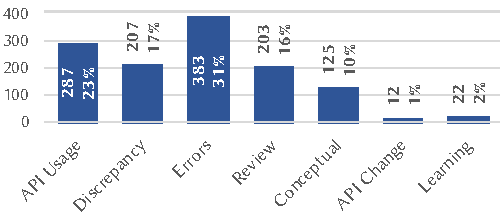
\includegraphics[width=.6\linewidth]{beyerclass}
\caption[Distributions of the types of questions raised]{Distribution of the types of questions raised.}
\label{semotion2021:fig:beyer-classifications}
\end{figure}

\Cref{semotion2021:fig:beyer-classifications} displays the overall distribution of question types from the \SEMNumTotalNonNoisePosts{} posts after applying noise-filtering and majority ruling to our original \SEMNumTotalPostsFromSO{} questions extracted. It is evident that developers ask issues predominantly related to \glsac{api} errors when using \glspl{cvs} and, additionally, how they can use the \glsac{api} to implement specific functionality. There are few questions related to version issues or self-learning. For further discussion into these results, we refer to \citep{Cummaudo:2020icse}.

\begin{table}[th]
\caption[Frequency of emotions per question type]{Frequency of emotions per question type.}
\label{semotion2021:tab:emotion-freq}
\footnotesize
\tablefit{\begin{tabular}{l|ccccccc|c}

\toprule
\textbf{Question Type}&
\textbf{Fear}&
\textbf{Joy}&
\textbf{Love}&
\textbf{Sadness}&
\textbf{Surprise}&
\textbf{Anger}&
\textbf{No Emotion}&
\textbf{Total}\\
\midrule
\glsac{api} Usage&47&22&34&17&59&13&136&328\\
Discrepancy&35&12&17&7&46&20&105&242\\
Errors&73&34&23&21&47&23&207&428\\
Review&35&16&15&16&42&14&95&233\\
Conceptual&27&9&10&8&21&5&61&141\\
\glsac{api} Change&4&2&2&1&1&1&5&16\\
Learning&3&4&2&0&4&0&11&24\\
\midrule
Total&224&99&103&70&220&76&620&1412\\
\bottomrule
\end{tabular}}
\end{table}

\Cref{semotion2021:tab:emotion-freq} displays the frequency of questions that were classified by EmoTxt when compared to our classification of question types. \cref{semotion2021:fig:emotion-dist} presents the emotion data proportionally across each type of question. In total, \SEMNumEmotionsDetected{} emotions were detected within the \SEMNumTotalNonNoisePosts{} non-noisy posts, and \SEMNumNoEmotionsDetected{} questions where EmoTxt predicted  \textit{No Emotion} for all the emotion classification runs.
Of the \SEMNumEmotionsDetected{} questions with emotion detected, \SEMNumQuestionsTwoEmo{} questions had two emotions predicted, \SEMNumQuestionsThreeEmo{} questions had three emotions detected, and \SEMNumQuestionsFourEmo{} question\footnote{See \url{http://stackoverflow.com/q/55464541}.} had four emotions detected (\textit{Surprise}, \textit{Sadness}, \textit{Joy} and \textit{Fear}). 

\textbf{\textit{No Emotion} was the most prevalent across all question types}, which is consistent with the findings of the Collab group during the training of the EmoTxt classifier. The next highest set of emotive questions are found in the second and fourth largest samples (\textit{Review} at 203 posts, and \textit{\glsac{api} Usage} at 287 posts); therefore, higher proportions of emotion is not necessarily correlated to sample size. (Note that the broad distribution of emotions under \textit{\glsac{api} Change} is not representative, as only 12 questions (1\%) were classified this issue type.)

Unsurprisingly, \textit{Discrepancy}-based questions---indicative of the frustrations developers face when the \glsac{api} does something unexpected---\textbf{had the highest proportion of \textit{Anger} detected}, at 8.26\%, compared to \textit{Anger}'s mean of \SEMPctAngerAverage{}.  \textbf{The two highest emotions, by average, were \textit{Fear} ($\mu=$\SEMPctFearAverage{}) and \textit{Surprise} ($\mu=$\SEMPctSurpriseAverage{})}. In contrast, to our surprise, \textbf{the two least-detected emotions reported by EmoTxt were \textit{Sadness} ($\mu=$\SEMPctSadnessAverage{}) and \textit{Anger} ($\mu=$\SEMPctAngerAverage{})}. \textbf{\textit{Joy} and \textit{Love} were roughly the same}, and fell in between the two proportion ends, with means of \SEMPctJoyAverage{} and \SEMPctLoveAverage{}, respectively.

\begin{table*}[t!]
\caption[Inter-rater agreement between human and automatic classification]{Inter-rater agreement between humans ($R_{1..3}$) and EmoTxt ($E$) and indicative guidelines of strength.}
\label{semotion2021:tab:irr-results}
\footnotesize
\tablefit{\begin{tabular}{l|cccc|cccc}
\toprule
\textbf{Emotion}&
$\mathbf{C_{\kappa}(R_{1},R_{2})}$&
$\mathbf{C_{\kappa}(R_{1},R_{3})}$&
$\mathbf{C_{\kappa}(R_{2},R_{3})}$&
$\mathbf{L_{\kappa}(R_{1..3})}$&
$\mathbf{C_{\kappa}(R_{1},E)}$&
$\mathbf{C_{\kappa}(R_{2},E)}$&
$\mathbf{C_{\kappa}(R_{3},E)}$&
$\mathbf{L_{\kappa}(R_{1..3},E)}$\\
\midrule
Love&0.30~\textit{Fair}&0.17~\textit{Slight}&0.04~\textit{Slight}&\textbf{0.17~\textit{Slight}}&0.37~\textit{Fair}&0.27~\textit{Fair}&0.05~\textit{Slight}&\textbf{0.20~\textit{Slight}}\\
Joy&0.21~\textit{Fair}&0.16~\textit{Slight}&0.57~\textit{Fair}&\textbf{0.31~\textit{Fair}}&0.1~\textit{Slight}&0.07~\textit{Slight}&-0.01~\textit{Poor}&\textbf{0.18~\textit{Slight}}\\
Surprise&0.21~\textit{Fair}&0.13~\textit{Slight}&0.15~\textit{Slight}&\textbf{0.16~\textit{Slight}}&0.17~\textit{Slight}&0.04~\textit{Slight}&0.06~\textit{Slight}&\textbf{0.13~\textit{Slight}}\\
Sadness&0.11~\textit{Slight}&0.05~\textit{Slight}&0.01~\textit{Slight}&\textbf{0.05~\textit{Slight}}&0.09~\textit{Slight}&0.04~\textit{Slight}&0.02~\textit{Slight}&\textbf{0.05~\textit{Slight}}\\
Fear&0.19~\textit{Slight}&0.22~\textit{Fair}&0.36~\textit{Fair}&\textbf{0.26~\textit{Fair}}&-0.02~\textit{Poor}&-0.06~\textit{Poor}&0.01~\textit{Slight}&\textbf{0.12~\textit{Slight}}\\
Anger&0.19~\textit{Slight}&0.19~\textit{Slight}&0.07~\textit{Slight}&\textbf{0.15~\textit{Slight}}&0.13~\textit{Slight}&0.16~\textit{Slight}&0.03~\textit{Slight}&\textbf{0.13~\textit{Slight}}\\
No Emotion&0.30~\textit{Fair}&0.16~\textit{Slight}&0.09~\textit{Slight}&\textbf{0.18~\textit{Slight}}&0.25~\textit{Fair}&0.06~\textit{Slight}&0.04~\textit{Slight}&\textbf{0.15~\textit{Slight}}\\
\bottomrule
\end{tabular}}
\end{table*}

As shown in \cref{semotion2021:tab:irr-results}, results from our reliability analysis between human raters indicated subjectivity in emotion interpretation. Guidelines of indicative strengths of agreement are provided by~\citet{Landis:1977kv}, where $\kappa \leq 0.00$ is \textit{poor} agreement, $0.00 < \kappa \leq 0.20$ is \textit{slight} agreement and $0.20 < \kappa \leq 0.40$ is \textit{fair} agreement. Our assessments across the 300 questions indicate slight agreement for \textit{Love}, \textit{Surprise}, \textit{Sadness}, \textit{Anger} and \textit{No Emotion}, and fair agreement for \textit{Joy} and \textit{Fear}. When combining human raters and EmoTxt, the inter-rater agreement was slight across all emotions.  

\begin{figure}[t!]
\centering
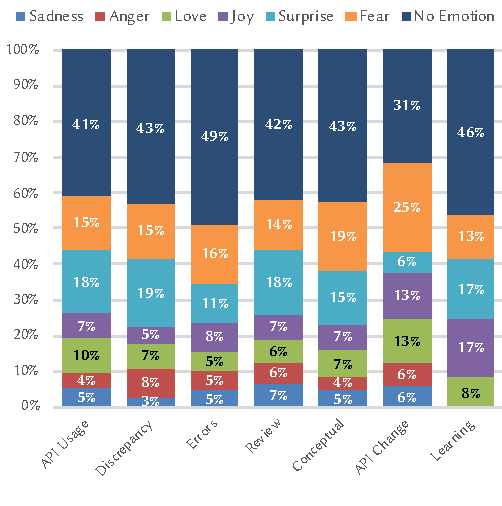
\includegraphics[width=.6\linewidth]{emotionproportion}
\caption[Proportions of emotions per question type]{Proportion of emotions per question type.}
\label{semotion2021:fig:emotion-dist}
\end{figure}

\afterpage{\begin{landscape}
\begin{table*}
\centering
\caption[Sample Stack Overflow questions with emotions identified]{Sample of various question types ([$Q$]) against emotion(s) identified by EmoTxt ([$E$]) and the three raters ([$R_{1..3}$]).}
\label{semotion2021:table:SampleQuestions}
\small
\tablefitlandscape{1}{\begin{tabular}{p{1\linewidth}p{0.2\linewidth}}
\toprule
\textbf{Question ID and Quote}&
\textbf{Classifications}\\

\midrule

\textbf{51444352}:~\textit{``I'm pretty sure I set up my IAM role appropriately (I literally attached the ComprehendFullAccess policy to the role) and the Cognito Pool was also setup appropriately (I know this because I'm also using Rekognition and it works with the IAM Role and Cognito ID Pool I created) and yet every time I try to send a request to AWS Comprehend I get the error... Any idea of what I can do in this situation?''}& 
[$Q$]:~Errors\newline
[$E$]:~Joy\newline
[$R_{1}$]:~Surprise\newline
[$R_{2}$]:~Surprise\newline
[$R_{3}$]:~Anger\medskip\\

{\textbf{53117918}:~\textit{``Ok so I have been stuck here for about more than a week now and I know its some dumb mistake. Just can't figure it out. I am working on a project that is available of two platforms, Android \& iOS. Its sort of a facial recognition app... Is there anything I need to change? Is there any additional setup I need to do to make it work?Please let me know. Thanks.''}}&
[$Q$]:~Discrepancy\newline
[$E$]:~Love, Surprise, Anger\newline
[$R_{1}$]:~Sadness, Anger\newline
[$R_{2}$]:~Sadness, Anger\newline
[$R_{3}$]:~Anger\medskip\\

\textbf{52829583}:~\textit{``I was trying to make the google vision OCR regex searchable... it fails when there is the text of other languages.It's happening because I have only English characters in google vision word component as follows.As I can't include characters from all the languages, I am thinking to include the inverse of above... So where can I find ALL THE SPECIAL CHARACTERS WHICH ARE IDENTIFIED AS A SEPARATE WORD BY GOOGLE VISION? Trial and error, keep adding the special characters I find is one option. But that would be my last option.''}&
[$Q$]:~Review\newline
[$E$]:~Anger\newline
[$R_{1}$]:~Joy, Anger\newline
[$R_{2}$]:~Anger\newline
[$R_{3}$]:~Surprise\medskip\\

\bottomrule
\end{tabular}}
\end{table*}\end{landscape}}

\section{Discussion}\label{semotion2021:sec:discussion}

\textbf{RQ1:} Our findings indicate that \citet{shaver1987}'s six basic emotions are detected in our questions. However, the majority of questions (\SEMPctNoEmotionAverage{}) were classified by EmoTxt as \textit{No Emotion}. It is reasonable to conclude that developers express \textit{some} emotive language in \gls{cvs} questions (the top three being \textit{Surprise}, \textit{Fear}, and \textit{Love}), but a little under half of all questions show no emotion at all. This study set out to explore whether the emotions in these questions can highlight issues with the service. We first need to have confidence in being able to identify these emotions. EmoTxt's results show that emotional analysis of \gls{so} questions is a \textit{partially reliable} indicator to identify developers' frustration with \glspl{cvs}. We can identify certain frustrations in \textit{some} questions, which may lead to aspects of improvement in \glspl{cvs}.  However, while some emotions may assist in identifying potential improvements for cloud vendors, not all questions will be considered due to their non-emotive language. The approach must thus be used in conjunction with other approaches to ensure that \textit{all} questions are considered. A different classifier trained on emotive \gls{so} questions may lead to different results. We leave such exploration open to future work. Making actual service improvements is a task we leave open to future research.

\textbf{RQ2:} Emotions present in different types of questions classified vary, the greatest variation being in \textit{\glsac{api} Change-} and \textit{Learning}-type questions. However, these two discrepancies are a result of limited sample size; 12 and 22 questions, respectively. Thus, if we consider only the other five question types, there are distinct patterns where certain emotions are strongest. Developers express the greatest fear in \textit{Conceptual} questions, where such emotive language likely accounts for a gap in the developer's theoretical understanding behind computer vision techniques, supporting our earlier work \citep{Cummaudo:2020icse}. The greatest amount of \textit{Surprise} and \textit{Anger} is in \textit{Discrepancy} questions, since the \glsac{api} is not behaving as the developer anticipates. Some emotions are harder to decipher. EmoTxt classified \SEMPctLoveAverage{} of questions as \textit{Love} across all of the different question types, most prevalently in the \textit{\glsac{api} Usage} questions. We expected this emotion to be least expressed by developers when they encounter issues. Thus, while the type of question will entail more or fewer emotions than others, \textit{interpreting} the reasons behind varying emotions is the more challenging factor. As it is impossible to follow-up with the authors of these questions and decipher the reasons for their emotional state, future studies with variant techniques could be guided by our results.

\textbf{RQ3:} Our findings in comparing manually annotated \gls{so} posts and automatic classification revealed substantial discrepancies. \Cref{semotion2021:table:SampleQuestions} provides some sample questions. The subset of questions analysed by our three raters do not indicate the automatic (EmoTxt) emotion. Upon manual inspection of the text an introspection of the dataset sheds some light on this. For example, the first question in \cref{semotion2021:table:SampleQuestions} shows no indication of \textit{Joy}, but EmoTxt classifies it to this emotion. Phrases like \textit{``I'm \textbf{pretty} sure...''} could be the reason why poor classification occurred, where words like ``pretty'' are associated with \textit{Joy}, albeit in a completely different context. It seems more likely the developer is experiencing a confusing situation and thus {[$R_{1}$]} and {[$R_{2}$]} noted \textit{Surprise}.  Similarly, in the second question presented in \cref{semotion2021:table:SampleQuestions}, EmoTxt classifies \textit{Love}, \textit{Surprise}, and \textit{Anger}. It is difficult to find an element of love or appreciation elsewhere in this context beyond closing remarks: \textit{``\textbf{Please} let me know. \textbf{Thanks}.''}. Moreover, the disparity between EmoTxt and the agreed emotions between the first two reviewers shows that EmoTxt cannot detect the frustration (\textit{Anger}) in the developer's tone, evident in their opening sentence, \textit{``I have been \textbf{stuck here} for about more than a week and I know it is some \textbf{dumb mistake}.''}. Our results indicate that further work is needed to refine EmoTxt when it is applied in new domains, like \gls{cvs} Q\&A. As highlighted by~\citet{curumsing2017}, the divergence of opinions with regards to an emotion classification model proposed by theorists raises doubts to the foundations of basic emotions. Most studies of  emotion mining from text use existing general purpose emotion frameworks from psychology~\citep{Ondrej:2016, ortu2016, novielli2018}, none tuned for the software engineering domain.

\textbf{RQ4:} Given the complexity and subjectivity of emotions~\citep{curumsing2017}, the efforts by the Collab team in automating emotions from \gls{so} posts is commendable. However, as our results have shown, agreement between a group of diverse individual raters indicates substantial subjectivity in the interpretation of emotions on \gls{so}. Without the use of reconciliation discussions to merge disparate emotional interpretations, our findings suggest that individuals will classify results based on their own personal biases.  Can classification of emotions in \gls{so} be fully automated? The alternative of having human raters is expensive and time consuming. Should we therefore work towards a mid-way solution?  One area of exploration is to reproduce classifications of emotions on the EmoTxt training dataset without reconciliation discussions and assess the overall reliability in the results.



\section{Threats to Validity}\label{semotion2021:sec:threats}

%\subsection{Internal validity} 
\subsection{Internal Validity} The \textit{\glsac{api} Change} and \textit{Learning} question types were few in sample size (only 12 and 22 questions, respectively). The emotion  proportion distribution of these question types are  quite different to the others.  Given the low number of questions, the sample is too small to make confident assessments. Moreover, 475 of the question types were classified by a single rater; a reliability analysis on these posts would be warranted. Lastly, our classifications of~\citeauthor{Beyer:2018fm}'s question type taxonomy was single-label; a multi-labelled approach may work better, however analysis of results would become more complex. A multi-labelled approach would be indicative for future work.

\subsection{External Validity} EmoTxt was trained on questions, answers and comments, however our dataset contained questions only. It is likely that our results may differ if we included other discussion items, however we wished to understand the emotion within developers' \textit{questions} and classify the question based on the question classification framework by~\citet{Beyer:2018fm}. Moreover, this study has only assessed frustrations within the context of a concrete domain; intelligent \glspl{cvs}. The generalisability of this study to other intelligent services, such as natural language processing services, or conventional web services, may be different. Furthermore, we only assessed four popular \glspl{cvs}; expanding the dataset to include more services, including non-English ones, would be insightful. We leave this to future work.

\subsection{Construct Validity} Some posts extracted from \gls{so} were false positives. Whilst flagged for removal, we cannot guarantee that all false positives were removed. Furthermore, \gls{so} is known to have questions that are either poorly worded or poorly detailed, and developers sometimes ask questions without doing any preliminary investigation. This often results in down-voted questions. We did not remove such questions which may influence the measurement of our results.

\section{Conclusion}\label{semotion2021:sec:conclusion}

In prior work~\citep{Cummaudo:2020icse}, we identified types of issues asked on Stack Overflow (\gls{so}) about four popular \glspl{cvs}.\textsuperscript{\ref{semotion2021:ftne:list-of-services}} Our ultimate goal is to prioritise which of these types of issues are worth addressing by cloud service vendors to effect useful improvements. To judge emotive Q\&A discussion of such services we trialled a pre-trained emotion classifier trained on \gls{so} posts. This tried to determine which of these issues have the strongest emotions, since prior work has demonstrated that emotions can affect developer productivity \citep{murgia2014, ortu2016, gachechiladze2017}. We identified that EmoTxt did not classify any emotions to \SEMPctNoEmotionAverage{} of the \SEMNumTotalPostsFromSO{} \gls{so} questions curated in \citep{Cummaudo:2020icse}. Of the questions that did appear to express emotive language (according to EmoTxt), we found that the distributions of emotions varied according to the different types of questions posed. Given that emotions are subjective~\citep{curumsing2017}, three raters  performed an inter-rater reliability analysis on the results of EmoTxt against a random sample of 300 posts, following the guidelines used to label data in EmoTxt~\citep{novielli2018}. Despite strictly adhering to these guidelines, we found that we could not find strong agreement between the three raters and EmoTxt nor indeed amongst the three raters themselves. Our results suggest EmoTxt classification does not generalise into new domains, such as computer vision Q\&A, due to subjectivity bias.

Consistent with prior work~\citep{lin2018sentiment}, our results demonstrate that certain machine-learnt classifiers are not fully reliable for emotion classification in \gls{so}. While manual assignment of emotions is an arduous and time-consuming process, following strict guidelines (i.e., \citep{novielli2018}) still yields subjectivity in the emotions classified. As our results highlight, applying a pre-trained emotional classifier in a new domain, such as \glspl{cvs}, will yield subjectivity issues and thus generalise poorly.